%!TEX root = ../template.tex
%%%%%%%%%%%%%%%%%%%%%%%%%%%%%%%%%%%%%%%%%%%%%%%%%%%%%%%%%%%%%%%%%%%%
%% chapter4.tex
%% NOVA thesis document file
%%
%% Chapter with lots of dummy text
%%%%%%%%%%%%%%%%%%%%%%%%%%%%%%%%%%%%%%%%%%%%%%%%%%%%%%%%%%%%%%%%%%%%

\typeout{NT FILE chapter4.tex}%


\chapter{Scan, Point Cloud Processing, and CAD Model}
\label{cha:digi}


\section{Scanning Process of the Compressor Blade}
\label{sec:scan}

The scanning of the compressor blade marked the initial phase of this work, aiming to generate a precise and detailed digital model of its complex geometry.
The scanning process was designed to encompass all necessary surfaces while minimizing errors and distortions.
Throughout this process, two main software tools were used: VXelements, for scan acquisition and initial alignment, and VXmodel, for advanced mesh editing and preparation for CAD reconstruction.

In the initial approach, a fixed table with pre-positioned targets was used, as shown in Figure~\ref{fig:setupinicial}, where the blade was placed and the operator moved around the part with the scanner, capturing different angles to ensure full surface coverage.

\begin{figure}[H]
    \centering
    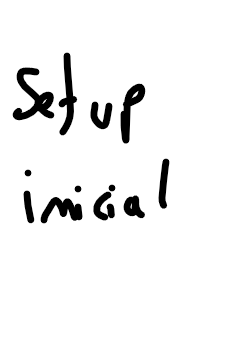
\includegraphics[width=0.1\textwidth]{setupinicial}
    \caption{Initial scanning setup with fixed table and stationary blade.}
    \label{fig:setupinicial}
\end{figure}


A technician from the Dimensional Inspection department at \gls{TAP} carried out the scan using the Creaform HandyScan, a handheld 3D scanner. 
The targets placed on the table served as reference points for the scanner's software, allowing it to maintain continuous alignment and improve the overall accuracy of the scanning process.
For this acquisition, a resolution of 0.008 inches was selected, although the HandyScan is capable of reaching a resolution as fine as 0.004 inches, the chosen setting was deemed sufficient to accurately capture the blade’s geometry without significantly increasing the scan duration or file size.

For this first approach, scanning was performed with the blade placed in two different positions, as shown in Figure~\ref{fig:pospasinical}

\begin{figure}[H]
    \centering
    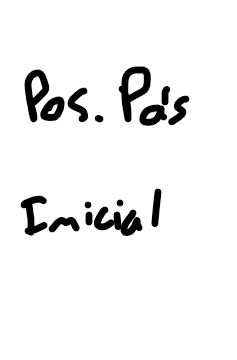
\includegraphics[width=0.1\textwidth]{pospasinicial}
    \caption{ Initial two blade positions used for scanning with the fixed table configuration.}
    \label{fig:pospasinical}
\end{figure}

The scanning process began by placing the blade in its first orientation on the fixed table with the targets already positioned. 
The scan was initiated in the VXelements software, and the operator proceeded to move the HandyScan 3D device manually around the blade, performing multiple passes to capture data from all visible surfaces. Throughout this stage, it was often necessary to adjust the scanner’s shutter speed in order to improve fluidity, reduce interruptions, and optimize surface acquisition in areas with challenging reflectivity.

Once the scanning pass was complete, the acquisition was stopped both on the HandyScan device and within the software. 
At this point, an initial cleanup was performed: the scan was filtered to remove noise, eliminate unwanted data such as the table, the targets, or stray reflections, and retain only a clean point cloud of the blade. This initial scan was saved, and a visual assessment was made to identify any areas of the blade geometry that were still missing or insufficiently captured.

The blade was then repositioned to expose the previously hidden surfaces, and a new scanning session was started. The process was repeated a second time.

Once both cleaned scans were available, an attempt was made to align them using the automatic best-fit alignment method. However, due to insufficient overlap or surface complexity, this method failed to produce a correct result. To overcome this, the software's manual alignment feature was used, which allows the selection of up to five corresponding points between the two scans. These user-defined reference points served as a basis for the alignment, enabling the software to successfully register the scans and merge them into a coherent and continuous point cloud.

The best-fit alignment method employs an iterative closest point algorithm, minimizes the squared distances between overlapping scan points, thereby achieving a seamless integration of the different scans into a single mesh.

After merging the individual scans into a single point cloud within VXelements, the dataset was exported to VXmodel for more advanced mesh processing. In this environment, dedicated tools were used to correct potential mesh defects such as irregularities, spikes, and holes. Once all scans were successfully merged into a continuous mesh, a global cleaning operation was performed to remove any extraneous points that did not belong to the blade geometry, including data captured unintentionally from the rotating table.
To address incomplete areas resulting from scanning limitations, the Fill Holes command was applied to reconstruct missing regions and generate a closed surface. This refined and watertight mesh served as a reliable foundation for developing the CAD model of the blade.

During the initial scanning attempts, several issues were encountered that impacted the completeness and efficiency of the process. Firstly, the operator was not given clear guidance on which surfaces of the blade were most critical to capture. As a result, the focus was placed predominantly on the airfoil region, while the platform areas were not sufficiently covered. This led to missing sections in the platform, which had to be reconstructed artificially during mesh processing in the post-scan phase.
One specific issue occurred during the scan of the sixth stage blade, where a non-functional surface was not properly captured. This was due to limited visibility in the two scanning orientations used in the initial setup, resulting in missing data in that region, as shown in Figure~\ref{fig:zonadanif} with a red mark.
Additionally, the highly reflective surface of the blade posed significant challenges for the scanner, especially in capturing fine details on certain faces. 
The fixed nature of the scanning table also introduced limitations, as the operator had to move around the part manually, often with constrained access and suboptimal scanning angles.
In some cases, fine particles such as talcum powder can be applied to reduce reflections and improve scan quality, although this method was not used in the present process.

\begin{figure}[H]
    \centering
    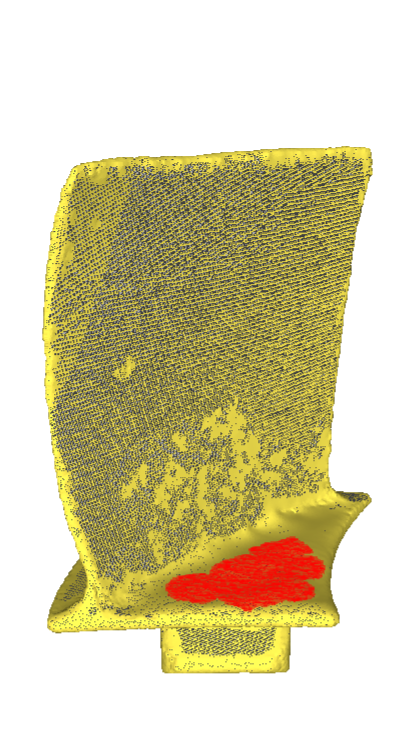
\includegraphics[width=0.4\textwidth]{zonadanif00}
    \caption{ Missing surface area in the sixth stage blade scan.}
    \label{fig:zonadanif}
\end{figure}

In light of these difficulties, a change in the scanning strategy was implemented. 
A new setup was introduced using a rotative table with integrated targets, allowing the blade to be rotated smoothly while the scanner remained in a stable position, as shown in Figure~\ref{fig:setupfinal}. 
This change improved both the fluidity of the scan and the consistency of surface acquisition. 

\begin{figure}[H]
    \centering
    
\includegraphics[width=0.1\textwidth]{setupfinal}
    \caption{Final scanning setup with rotative table and integrated targets.}
    \label{fig:setupfinal}
\end{figure}


Furthermore, the number of scanning stages was increased from two to three, allowing for more thorough coverage of the entire blade geometry and ensuring that critical areas, such as the platform, were adequately captured.
To specifically address the missing surface in the sixth stage blade, the third scanning position was performed with the blade placed vertically on the table surface, improving visibility and ensuring full data acquisition in that region.
The three scanning positions used in this final configuration are illustrated in Figure~\ref{fig:pospasfinal}.

\begin{figure}[H]
    \centering
    
\includegraphics[width=0.1\textwidth]{pospasfinal}
    \caption{ Final three blade positions used in the revised scanning approach.}
    \label{fig:pospasfinal}
\end{figure}

Finally, it should be noted that the leading and trailing edges of the blade exhibit several irregularities in the resulting mesh, as shown in Figure~\ref{fig:snapshot}. 
Due to the extremely thin geometry of these regions, the scan resolution did not produce a sufficiently dense set of points to represent them smoothly, resulting in a jagged and discontinuous appearance. 
Although these edges are relevant to the scope of this work, the observed irregularities do not critically affect the overall objectives. 
This limitation will be addressed and corrected in the following chapter, where the CAD reconstruction process is detailed.

\begin{figure}[H]
    \centering
    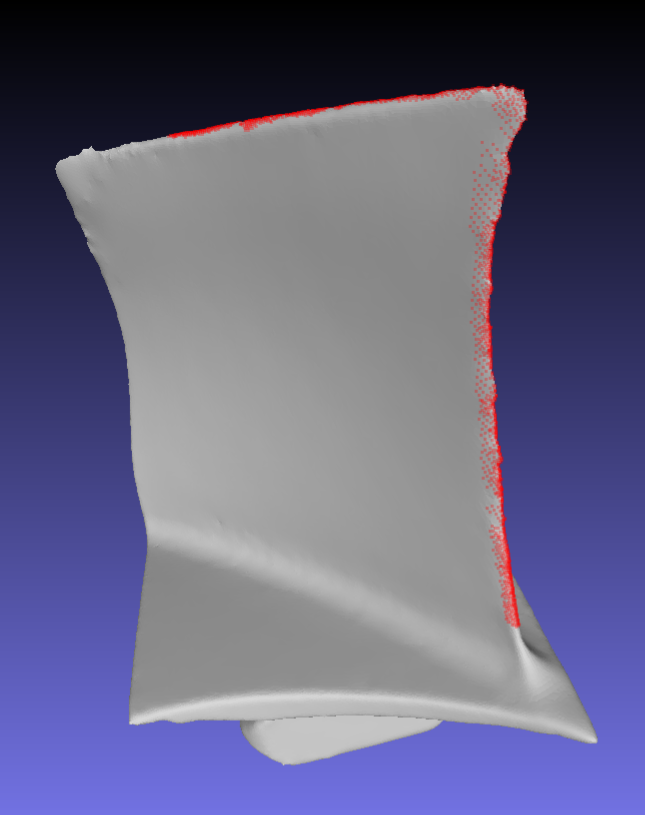
\includegraphics[width=0.4\textwidth]{snapshot00}
    \caption{ Irregularities in the leading and trailing edges of the scanned mesh caused by limited point density.}
    \label{fig:snapshot}
\end{figure}

In summary, the scanning process for the compressor blade involved multiple orientations, manual alignment using best-fit techniques, and detailed mesh refinement to obtain a high-quality digital representation. Despite some limitations and challenges, the resulting scans provided a robust and accurate basis for subsequent CAD modeling and geometric analysis. Figure~\ref{fig:scan1} shows the point cloud obtained from the scanning of the sixth stage blade.
\begin{figure}[H]
    \centering
    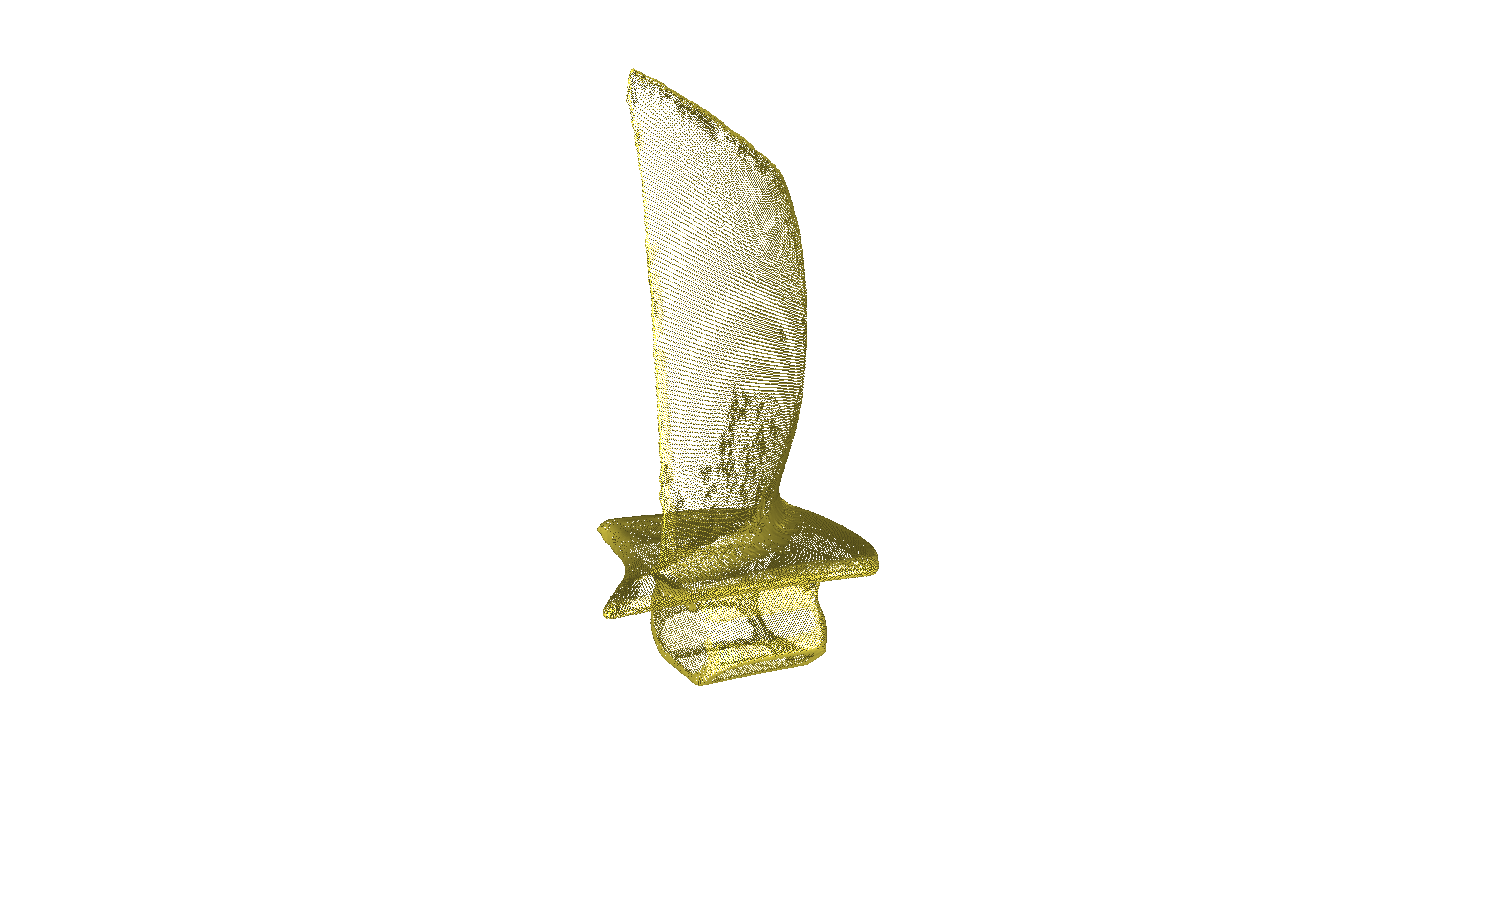
\includegraphics[width=0.4\textwidth]{scan1}
    \caption{Stage 6 Point Cloud}
    \label{fig:scan1}
\end{figure}

\section{Point Cloud Processing and CAD Model Creation}
\label{sec:cad}

To generate the CAD model from the scanned data, the point cloud was processed and imported into SolidWorks using the Xtract3D add-in. This tool facilitated working directly with the point cloud by enabling reference geometry creation and surface sculpting based on the scanned data.

Unlike traditional workflows where an STL file is imported as a surface body to optimize processing, Xtract3D allowed for direct manipulation of the point cloud without losing critical geometric information. This streamlined the modeling process, reducing the need for intermediate conversions and preserving the fidelity of the scanned data.

Using the Xtract3D slice feature, cross-sections were extracted from the point cloud, as represented in Figure~\ref{fig:slice}. This allows guiding the creation of accurate profiles and lofted surfaces that replicated the original blade geometry with high precision. By leveraging these tools, the CAD model was refined iteratively to match the scanned data while ensuring manufacturability and compatibility with further analysis.

\begin{figure}[H]
    \centering
    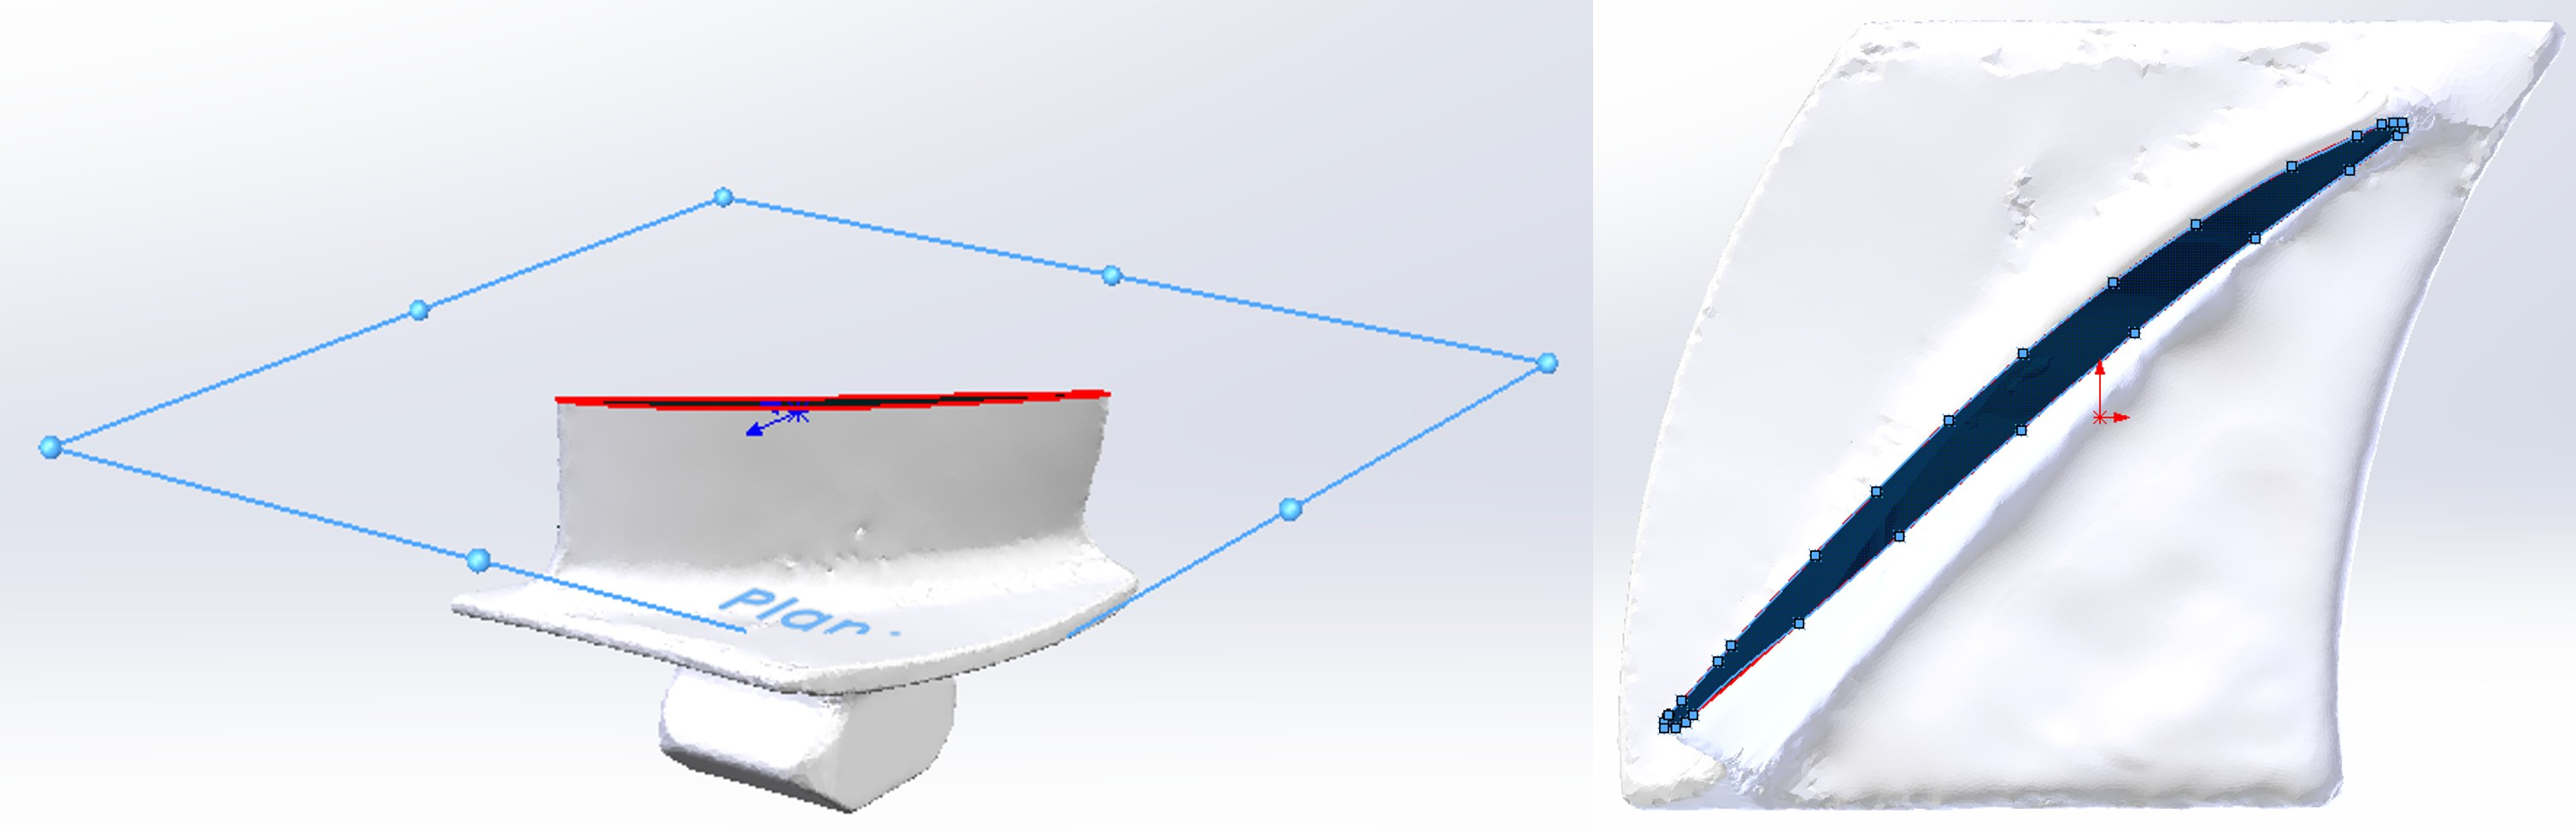
\includegraphics[width=0.8\textwidth]{slice}
    \caption{Mesh and CAD Comparison}
    \label{fig:slice}
\end{figure}

As illustrated in Figure~\ref{fig:compare.png}, this process enables the generation of an accurate CAD model from the scanned data.

\begin{figure}[H]
    \centering
    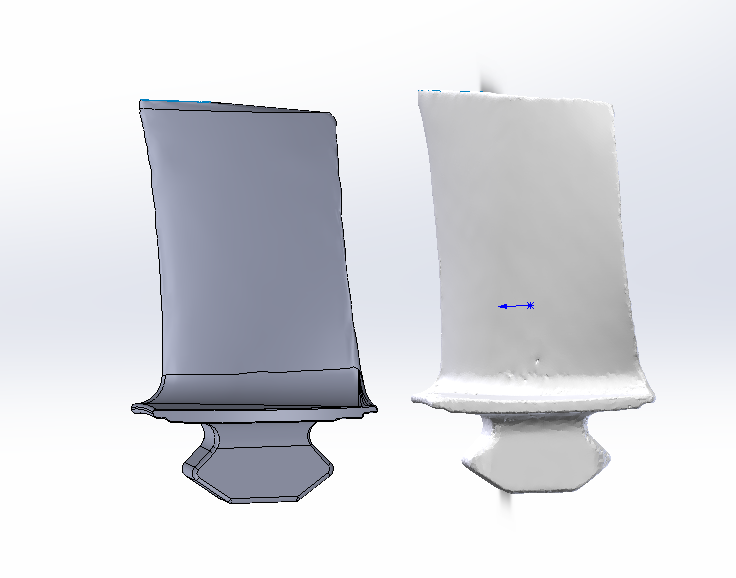
\includegraphics[width=0.5\textwidth]{compare.png}
    \caption{Mesh and CAD Comparison}
    \label{fig:compare.png}
\end{figure}

In the next section, the accuracy of the generated model will be evaluated against the scanned blade, accompanied by additional analyses, in order to ensure a parametric model accurate enough to support the development of this dissertation.
